\documentclass{beamer}
\usepackage{ctex}
\usepackage{times}
\usepackage{multicol}
\usepackage{multirow}
\usetheme{Warsaw}
%\usecolortheme{beaver}     % use white-grey colour style

% This is only inserted into the PDF information catalog. Can be left out.
\subject{presentation}
\keywords{example}

%% ======================================================
%%     preamble
%% ======================================================
\title{使用\LaTeX{}+Beamer创建演示文稿的简单例程}
\subtitle{Making Slides with Beamer}
%% for single author
%\author{张三}
%\institute{XXX大学}

%% for multi-authors
\author
{J.~LaTeX\inst{1} \and M.~Beamer\inst{2}}
 
\institute
{
  \inst{1}
  机械工程学院~南京理工大学
  \and
  \inst{2}
  Department of Aerospace Engineering\\
  University of Bristol
}
\date{\today}

\logo{
\includegraphics[height=0.09\textwidth]{./logo/njust_logo}}


%% ======================================================
\begin{document}

%% ++++++++++++++++++++++++++++++++++++++++++++++++++++++
%% title page
%% ++++++++++++++++++++++++++++++++++++++++++++++++++++++
\begin{frame}
  \titlepage
\end{frame}

%% ++++++++++++++++++++++++++++++++++++++++++++++++++++++
%%     Table of Contents
%% ++++++++++++++++++++++++++++++++++++++++++++++++++++++
\begin{frame}
    \frametitle{Contents}
    %\tableofcontents
    %% 显示1-4section,不显示subsection
    \tableofcontents[hidesubsections,sections={<1-4>}]
\end{frame}

%% ++++++++++++++++++++++++++++++++++++++++++++++++++++++
%%     main part
%% ++++++++++++++++++++++++++++++++++++++++++++++++++++++
%\section{文本与列表}
\begin{frame}
  \frametitle{关于\LaTeX{}和Beamer}
  \framesubtitle{关于\LaTeX{}}
  \begin{enumerate}
    \item<1-> 简单化的文本编辑工具;
    \item<2-> 完全兼容\LaTeX{}命令;
    \item<3-> 其实不明白,只是感兴趣。
  \end{enumerate}
\end{frame}

%% ++++++++++++++++++++++++++++++++++++++++++++++++++++++
%%      Tables
%% ++++++++++++++++++++++++++++++++++++++++++++++++++++++
%\section{表格、公式和图片}
\begin{frame}
  \frametitle{表格}
  \begin{table}
    \caption{时间表}
    \label{tab:times}
    \begin{tabular}{c|c|c|c}
      \hline
      % \multicolumn{2}{c}{\backslashbox{Name}{Numer}} &  \multicolumn{2}{c}{}\\ \hline
      \multirow{2}{*}{CleanEval} & \multirow{2}{*}{CleanEval-Eng} & training set & 60 \\ \cline{3-4} 
      \multirow{2}{*}{}          & \multirow{2}{*}{}              & evaluation set &   864 \\ \hline 
 
      \multirow{6}*{CETD} & NYTimes      & \multicolumn{2}{c}{100} \\ \cline{2-4} 
      \multirow{6}*{}     & Yahoo!       & \multicolumn{2}{c}{100} \\ \cline{2-4} 
      \multirow{6}*{}     & Wikipedia    & \multicolumn{2}{c}{100} \\ \cline{2-4}
      \multirow{6}*{}     & BBC          & \multicolumn{2}{c}{100} \\ \cline{2-4}
      \multirow{6}*{}     & Ars Technica & \multicolumn{2}{c}{100} \\ \cline{2-4}
      \multirow{6}*{}     & Chaos        & \multicolumn{2}{c}{200} \\ \hline 
    \end{tabular}
  \end{table}
\end{frame}

%% ++++++++++++++++++++++++++++++++++++++++++++++++++++++
%%      Equation & Figures
%% ++++++++++++++++++++++++++++++++++++++++++++++++++++++
\begin{frame}
\frametitle{图片}

\begin{figure}
\centering
   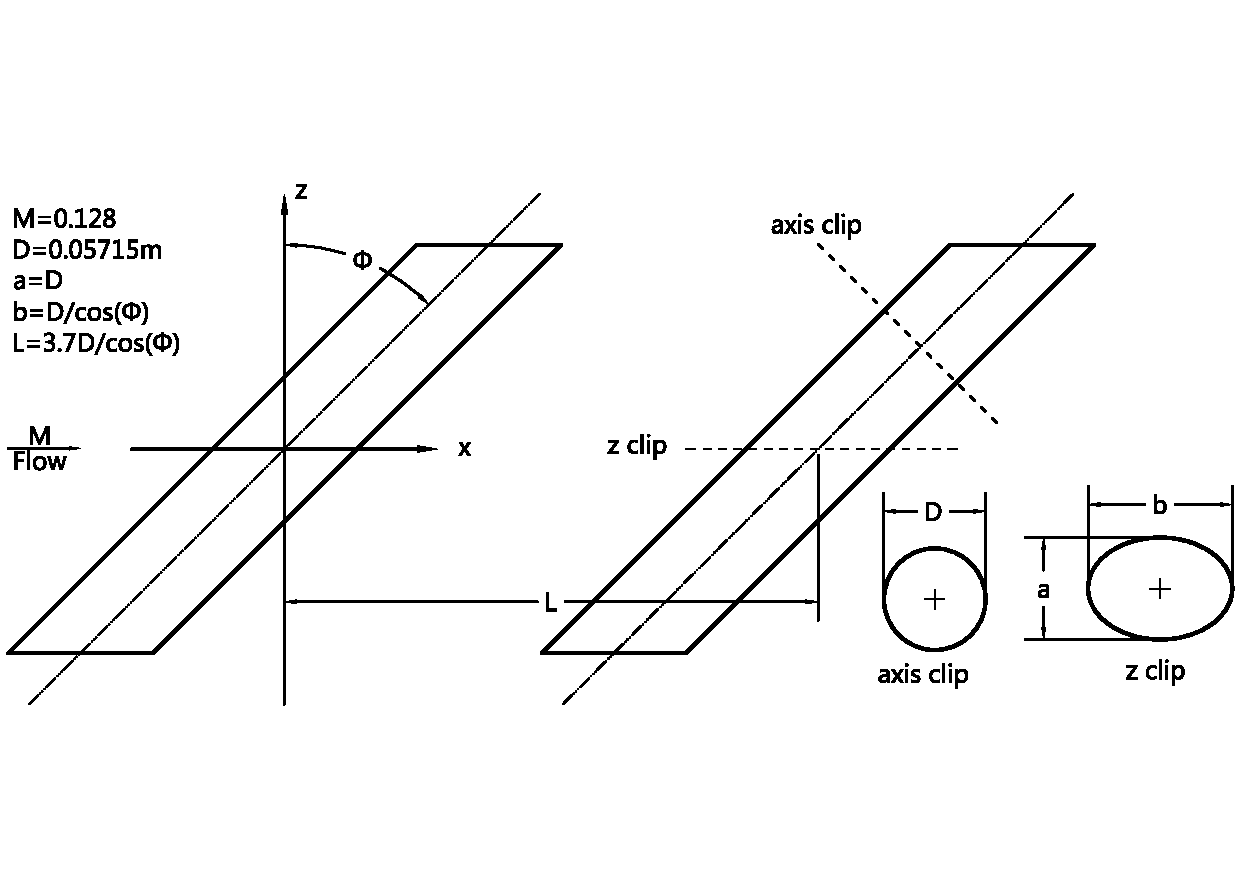
\includegraphics[height=6cm]{./img/Geom_pdf}
  \caption{插入一个pdf图片}
  \label{fig:visual}
\end{figure}

\end{frame}

%% ++++++++++++++++++++++++++++++++++++++++++++++++++++++
%%
%% ++++++++++++++++++++++++++++++++++++++++++++++++++++++
\begin{frame}
  \frametitle{框图与公式}
  \begin{theorem}
    There is no largest prime number.
    \begin{equation}
      \label{eqn:LBmodel}
      C_{L}=C_{L0}+C_{L\alpha }\left ( \frac{1+\sqrt{X}}{2} \right )\alpha 
    \end{equation}
  \end{theorem}

  \begin{proof}
  \begin{enumerate}
    \item<1-| alert@1> Suppose $p$ were the largest prime number.
    \item<2-> Let $q$ be the product of the first $p$ numbers.
    \item<3-> Then $q+1$ is not divisible by any of them.
    \item<1-> But $q + 1$ is greater than $1$, thus divisible by some prime number not in the first $p$ numbers.\qedhere
    \end{enumerate}
  \end{proof}

\end{frame}

%% ++++++++++++++++++++++++++++++++++++++++++++++++++++++
%%      Last Page
%% ++++++++++++++++++++++++++++++++++++++++++++++++++++++
\begin{frame}
Thank You!

\end{frame}

%% ++++++++++++++++++++++++++++++++++++++++++++++++++++++
%%      Reference Page
%% ++++++++++++++++++++++++++++++++++++++++++++++++++++++
\begin{frame}[allowframebreaks]{References} 
  \scriptsize
  \bibliographystyle{apalike}
  \bibliography{myRefs}
\end{frame}

\end{document}
%% ======================================================